\chapter{New Experimental Approaches Enabling the Continuous Monitoring of Gas Species in Hydrothermal Fluids}
\label{ch:methodological}

% ------------ 1st page ------------- %

\chaptermark{Chapter 2} % to change the headers
%\setcounter{figure}{0}
%\setcounter{table}{0}

Sébastien Giroud$^{1,2}$, Yama Tomonaga$^{1}$, Matthias S. Brennwald$^{1}$, \\
Naoto Takahata$^{3}$, Tomo Shibata$^{4}$, Yuji Sano$^{5}$, and Rolf Kipfer$^{1,2,6}$ \\

\noindent
This chapter has been published in \textit{Frontiers in Water}.\\
DOI: \url{10.3389/frwa.2022.1032094}

\blfootnote{\begin{flushleft}
$^{1}$Department of Water Resources and Drinking Water, Eawag, Dübendorf, Switzerland\\
$^{2}$Institute of Biogeochemistry and Pollutant Dynamics, ETH Zürich, Zurich, Switzerland\\
$^{3}$Atmosphere and Ocean Research Institute, The University of Tokyo, Kashiwa-shi, Japan\\
$^{4}$Institute for Geothermal Sciences, Kyoto University, Kyoto, Japan\\
$^{5}$Center for Advanced Marine Core Research, Kochi University, Kochi, Japan\\
$^{6}$Institute of Geochemistry and Petrology, ETH Zürich, Zurich, Switzerland\\

\end{flushleft}}

\vspace*{\fill}
\null{
\textcolor{gray}{
\footnotesize % Adjust size as needed
\noindent
\textbf{Acknowledgements}\\ 
PhD support for SG and open access funding provided by Eawag - Swiss Federal Institute of Aquatic Science and Technology.
We are grateful to Eline Mignot, Gabriele Bianchetti, and Jean-Marie Rouiller for providing us access to the hydrothermal wells in Lavey-les-Bains and valuable monitoring data. 
We thank André Défago for his help during the fieldwork in Lavey-les-Bains. 
We thank Tehnuka Ilanko, Johannes A. C. Barth, and Stephanie Musy for their time and effort to improve our initial version of the manuscript, and Dr Hugo Delottier for handling the manuscript. 
}}

% ------------ 2nd page ------------- %
\newpage
\noindent
\textbf{Abstract:} Hot thermal fluids flow through the Earth's crust and carry valuable information about the deep subsurface.
The monitoring of natural tracers transported in geothermal fluids, such as gases or ions, are relevant to better understand the geological processes in the Earth's subsurface and their relation to deep fluid dynamics.
Recently developed technologies (e.g., portable gas-equilibrium membrane-inlet mass spectrometry) allow for the continuous monitoring of gas species at a much higher temporal resolution than the sampling procedures commonly used, based on a few individual samples. 
However, the monitoring of gas species from hot thermal fluids still poses experimental challenges tied to unwanted water vapor condensation in the headspace of the separation module, which irremediably leads to clogging (e.g., of the connecting capillaries) and failure of the detection device. 
In this contribution, we present two new experimental methods that provide suitable technical conditions to measure gases, even in high temperature geothermal fluids, using a portable gas analyzer. 
Two sites with different thermal water temperatures (first one ranging from \SI{50}{\celsius} to \SI{65}{\celsius} and second one close to boiling temperature) were selected.
The first method was deployed on the thermal waters of Lavey-les-Bains (Vaud, Switzerland), for which we report results from October 2021.
The second method was used in Beppu (Oita Prefecture, Japan), for which we report results from April 2018.
Our results show that at both sites, our methods allow for continuous measurements of gas species (\ce{N2}, Ar, \ce{O2}, Kr, He, \ce{CH4}, \ce{CO2} and \ce{H2}) in thermal waters.
Furthermore, they show that the variability of gas emanation from the two sites can only be adequately described by measurements with high temporal resolution, which both methods allow. 

\section{Introduction}
Groundwater and other terrestrial fluids transport valuable information about deep fluid dynamics. 
Elemental and isotopic composition of terrestrial fluids can indicate the origin of the fluid or inform about possible routes the fluid has taken.
Furthermore, their elemental and isotopic composition can also respond to crustal events, such as earthquakes \citep{ide2020kumamoto}.
The natural variability in time and space of terrestrial fluids often cannot be reasonably characterized by isolated measurements. 
The characterization of natural variability requires a series of measurements at a sampling rate higher than the rate of natural variability in gas composition within the fluid (e.g., weekly to biweekly for a seasonal trend).  
This results in tedious laboratory work if conventional sampling protocols and measuring procedures are applied (i.e., off-site laboratory analysis, \cite{beyerle2000mass}).
Nevertheless, such in-depth knowledge of fluid dynamics in the Earth's crust is essential, as the crust has become of central interest in current societal energy transition processes, such as carbon sequestration, geothermal power generation, or geological deep storage of spent nuclear fuel.
Moreover, fluid dynamics could, at least on a conceptual level, inform about the potential relationship between fluid evolution and natural processes in the Earth's crust, such as volcanic or seismic activity. 

To characterize the variability of gas species in groundwater and terrestrial fluids, recent monitoring technologies have evolved toward more continuous measurements under in situ conditions (e.g., continuous \ce{^222Rn} monitoring in the coastal zone with RAD7, \cite{burnett2001radon}; continuous \ce{^220Rn} and \ce{^222Rn} monitoring in groundwater with RAD7, \cite{huxol2012radon}; continuous measurements of carbon dioxide and methane with cavity ring-down spectroscopy, \cite{chen2010picarro}; continuous monitoring of carbon dioxide with laser isotope spectrometer, \cite{frank2020co2}; continuous measurements of dissolved gases with continuous flow membrane inlet mass spectrometer, \cite{chatton2017continuous}; in situ denitrification tracing with gas-equilibrium membrane-inlet mass spectrometry, \cite{popp2020denitrifaction}; dissolved gases monitoring in groundwater with conventional membrane-inlet mass spectrometry, \cite{takahata1997continuous}, or with gas-equilibrium membrane-inlet mass spectrometry, \cite{maechler2013miniruedi}; in situ argon and helium monitoring with gas-equilibrium membrane-inlet mass spectrometry, \cite{roques2020helium}).
These available technologies allow gases to be measured in a quasi-continuous mode from both gaseous and liquid phases, often relying on specific semi-permeable membranes which allow separation of the dissolved gaseous phase from liquid phases. 
Whether the gases are sampled from a liquid or gas phase, available methods generally require matrices free of liquid water, that is, the analytical methods are sensitive to high water vapor partial pressure and the associated risk of water vapor condensation in the headspace of the module containing the gas-permeable membrane.
As the headspace fills up with water and no longer allows the proper separation of dissolved gases from the liquid phase, the inlet of a gas analyzer can draw in water and clog, especially if the gas analyzer uses capillaries to deliver gases to the mass spectrometer (e.g., OmniStar\textsuperscript{\tiny\textregistered} by Pfeiffer or miniRUEDI by Gasometrix).
Obtaining liquid-free matrices for gas analysis becomes even more challenging when monitoring gas species in geothermal fluids.
Both the exponential increase in water vapor saturation in the gas phase with increasing fluid temperature and the cooler surface of the membrane module that favors water vapor condensation in the headspace can quickly lead to clogging of the membrane module and inlet capillaries if those are used to inlet gases to the gas detector.

To overcome the challenge of water vapor condensation in the head-space and the clogging of the connecting capillaries, we present two different methods that have been developed to adapt the available monitoring schemes to geothermal waters and gases rich in water vapor.
In our case, we combined the developed experimental techniques specifically with a gas-equilibrium membrane-inlet mass spectrometer (miniRUEDI, \cite{brennwald2016portable}) as an analytical detector coupled to a gas-permeable membrane module (Liqui-Cel\textsuperscript{\tiny\texttrademark}, 3M\textsuperscript{\tiny\texttrademark}).
Nevertheless, we note that both methods can easily be adapted to any other detection method commonly used for continuous gas quantification based on the separation of dissolved gases from the liquid phase, where the condensation of water vapor in the headspace jeopardizes the proper functioning of the membrane module, and particularly to those based on capillaries for gas inlet.

Two sites were studied covering two different water temperature ranges. 
At the first site, different wells with temperatures ranging up to \SI{65}{\celsius} (Section \ref{sec:mod-high}) were accessible for continuous gas measurement in a thermal production well. 
At the second site, the water temperature was too high to be compatible with the temperature range specified for the separation membrane used.
Therefore, an alternative method was developed allowing gas quantification at fluid temperature exceeding \SI{65}{\celsius} (Section \ref{sec:high}).
In both cases, the specifically developed methods, which are described in the experimental subsections, provide a suitable framework for the continuous monitoring of gas species (\ce{N2}, Ar, \ce{O2}, Kr, He, \ce{CH4}, \ce{CO2} and \ce{H2}) from geothermal waters and other geothermal fluids.


\section{Study sites and methods}

\subsection{Study sites}
The first site, Lavey-les-Bains (Switzerland), is located in the Rhône Valley, where thermal water is abstracted from a gneiss formation of the Aiguilles Rouges alpine massif \citep{sonney2009numerical, sonney2012circulation}. 
The rocks are strongly fractured and allow groundwater to recharge and circulate deeply into the continental crust before reappearing at the central plain of the Rhône Valley.
The thermal water of Lavey-les-Bains has been suggested to recharge at the top of the Aiguilles Rouges massif, which is located west of the lower Rhône valley (approx. \SI{430}{\masl}) at high altitude (approx. 1000--\SI{3000}{\masl}) \citep{sonney2009numerical, sonney2012circulation}.
In Lavey-les-Bains, hot thermal water is abstracted from three deep wells (\SI{201}{\mbgl}, \SI{280}{\mbgl}, and \SI{516}{\mbgl}) that were drilled between 1970 and 1990 and supply the local thermal spa infrastructure.
The deepest borehole withdraws water at \SI{64}{\celsius}, which is fed by the underlying hydrothermal reservoir.

The second site is located in the Horita hot spring area in the city of Beppu on the Kyushu Island, Southwestern Japan.
In the area, fluids gush from a deep high temperature reservoir (250--\SI{300}{\celsius}, \cite{sturchio1996beppu, allis1989beppu}).
The analyzed monitoring well is hydraulically connected to the Horita-Asamigawa Fault Zone, which belongs to the Beppu–Shimabara graben.
In April 2016, the Beppu-Shimabara graben was particularly active at the Futagawa-Hinagu Fault Zone, which was responsible for the Kumamoto earthquakes (mainshock at magnitude 7.3, \cite{ide2020kumamoto}).
The Kumamoto earthquakes have been shown to have changed the gas composition of deep groundwaters, whereby higher \ce{^4He} concentrations and lower \ce{^3He}/\ce{^4He} ratios as the result of injection of radiogenic He from crustal rocks have been reported \citep{sano2016kumamoto}.  
This observation suggests that He and other geogenic gases have the potential to be used as indicators for seismic activity along active fault systems. 

\subsection{Portable mass spectrometer system}
At both study sites, the gas composition was continuously determined under field conditions over several weeks by using portable gas-equilibrium membrane-inlet mass spectrometry (miniRUEDI).
The device allows the quantification of the partial pressures of multiple gas species (e.g., He, Ar, Kr, \ce{N2}, \ce{O2}, \ce{CH4}, \ce{CO2}) in liquid or gaseous fluids \citep{brennwald2016portable}.
Major gas species are determined on a Faraday cup, and trace gases are analyzed on an electron multiplier detector.
The raw data obtained from the mass spectrometer were calibrated in terms of the partial pressures of the analyzed gases using ambient air \citep{porcelli2018noblegases} or a gas mixture (\SI{97}{\percent} \ce{N2}, \SI{1}{\percent} \ce{H2}, \SI{1}{\percent} \ce{CO2}, and \SI{1}{\percent} \ce{CH4}, \cite{tomonaga2019montterri}) as standards. 
Sample measurements were followed by calibrations using the two standards.
Standards were measured at least 6 times a day, as measurement conditions were rather stable over the period of the experiment \citep{brennwald2016portable}.
It should be noted that the calibration frequency can be increased in more variable environmental conditions.

The quantification of gas species in liquid phases by a gas analyzer commonly requires the separation of gases from the liquid phase. 
The gas-permeable membrane module (polypropuylene/polyurethane membrane, 3M\textsuperscript{\texttrademark} Liqui-Cel\textsuperscript{\texttrademark}) separates gases from the liquid phase.
The membrane operates such that the gas phase in the membrane module is at equilibrium with the gases dissolved in the thermal water that runs through the membrane module. 
A minimal water flow (\SI{1}{\litre\per\minute}) across the membrane module is required to reach proper equilibrium between the dissolved gas phase in thermal waters and the headspace of the membrane module. 
For common applications under typical ambient surface conditions (fluids with temperatures between 0-\SI{30}{\celsius}), the partial pressure of water vapor inside the membrane module is rather low and the condensation of water vapor in the headspace barely interferes with mid- and long-term quantification of gas species.

\subsection{Geothermal waters up to 65\textcelsius}\label{sec:mod-high}
Thermal waters degas once reaching the surface as result of the lower surface pressure and the high water temperature. 
Quantification of thermal water gases with conventional sampling techniques (e.g., copper tube sampling) is therefore problematic because the gas bubbles sampled along with the water may not be representative of the targeted water parcel.
In this case, the use of the membrane module is more appropriate because the headspace equilibrium across the membrane is not affected by the degassing, as both dissolved and free gases equilibrate with the headspace \citep{lightfoot2022noble}.
However, the high content of gaseous water in the headspace promotes the formation of liquid water, which leads to clogging of the headspace and the capillary inlet of the gas analyzer. 

\begin{figure}[ht!]
\begin{center}
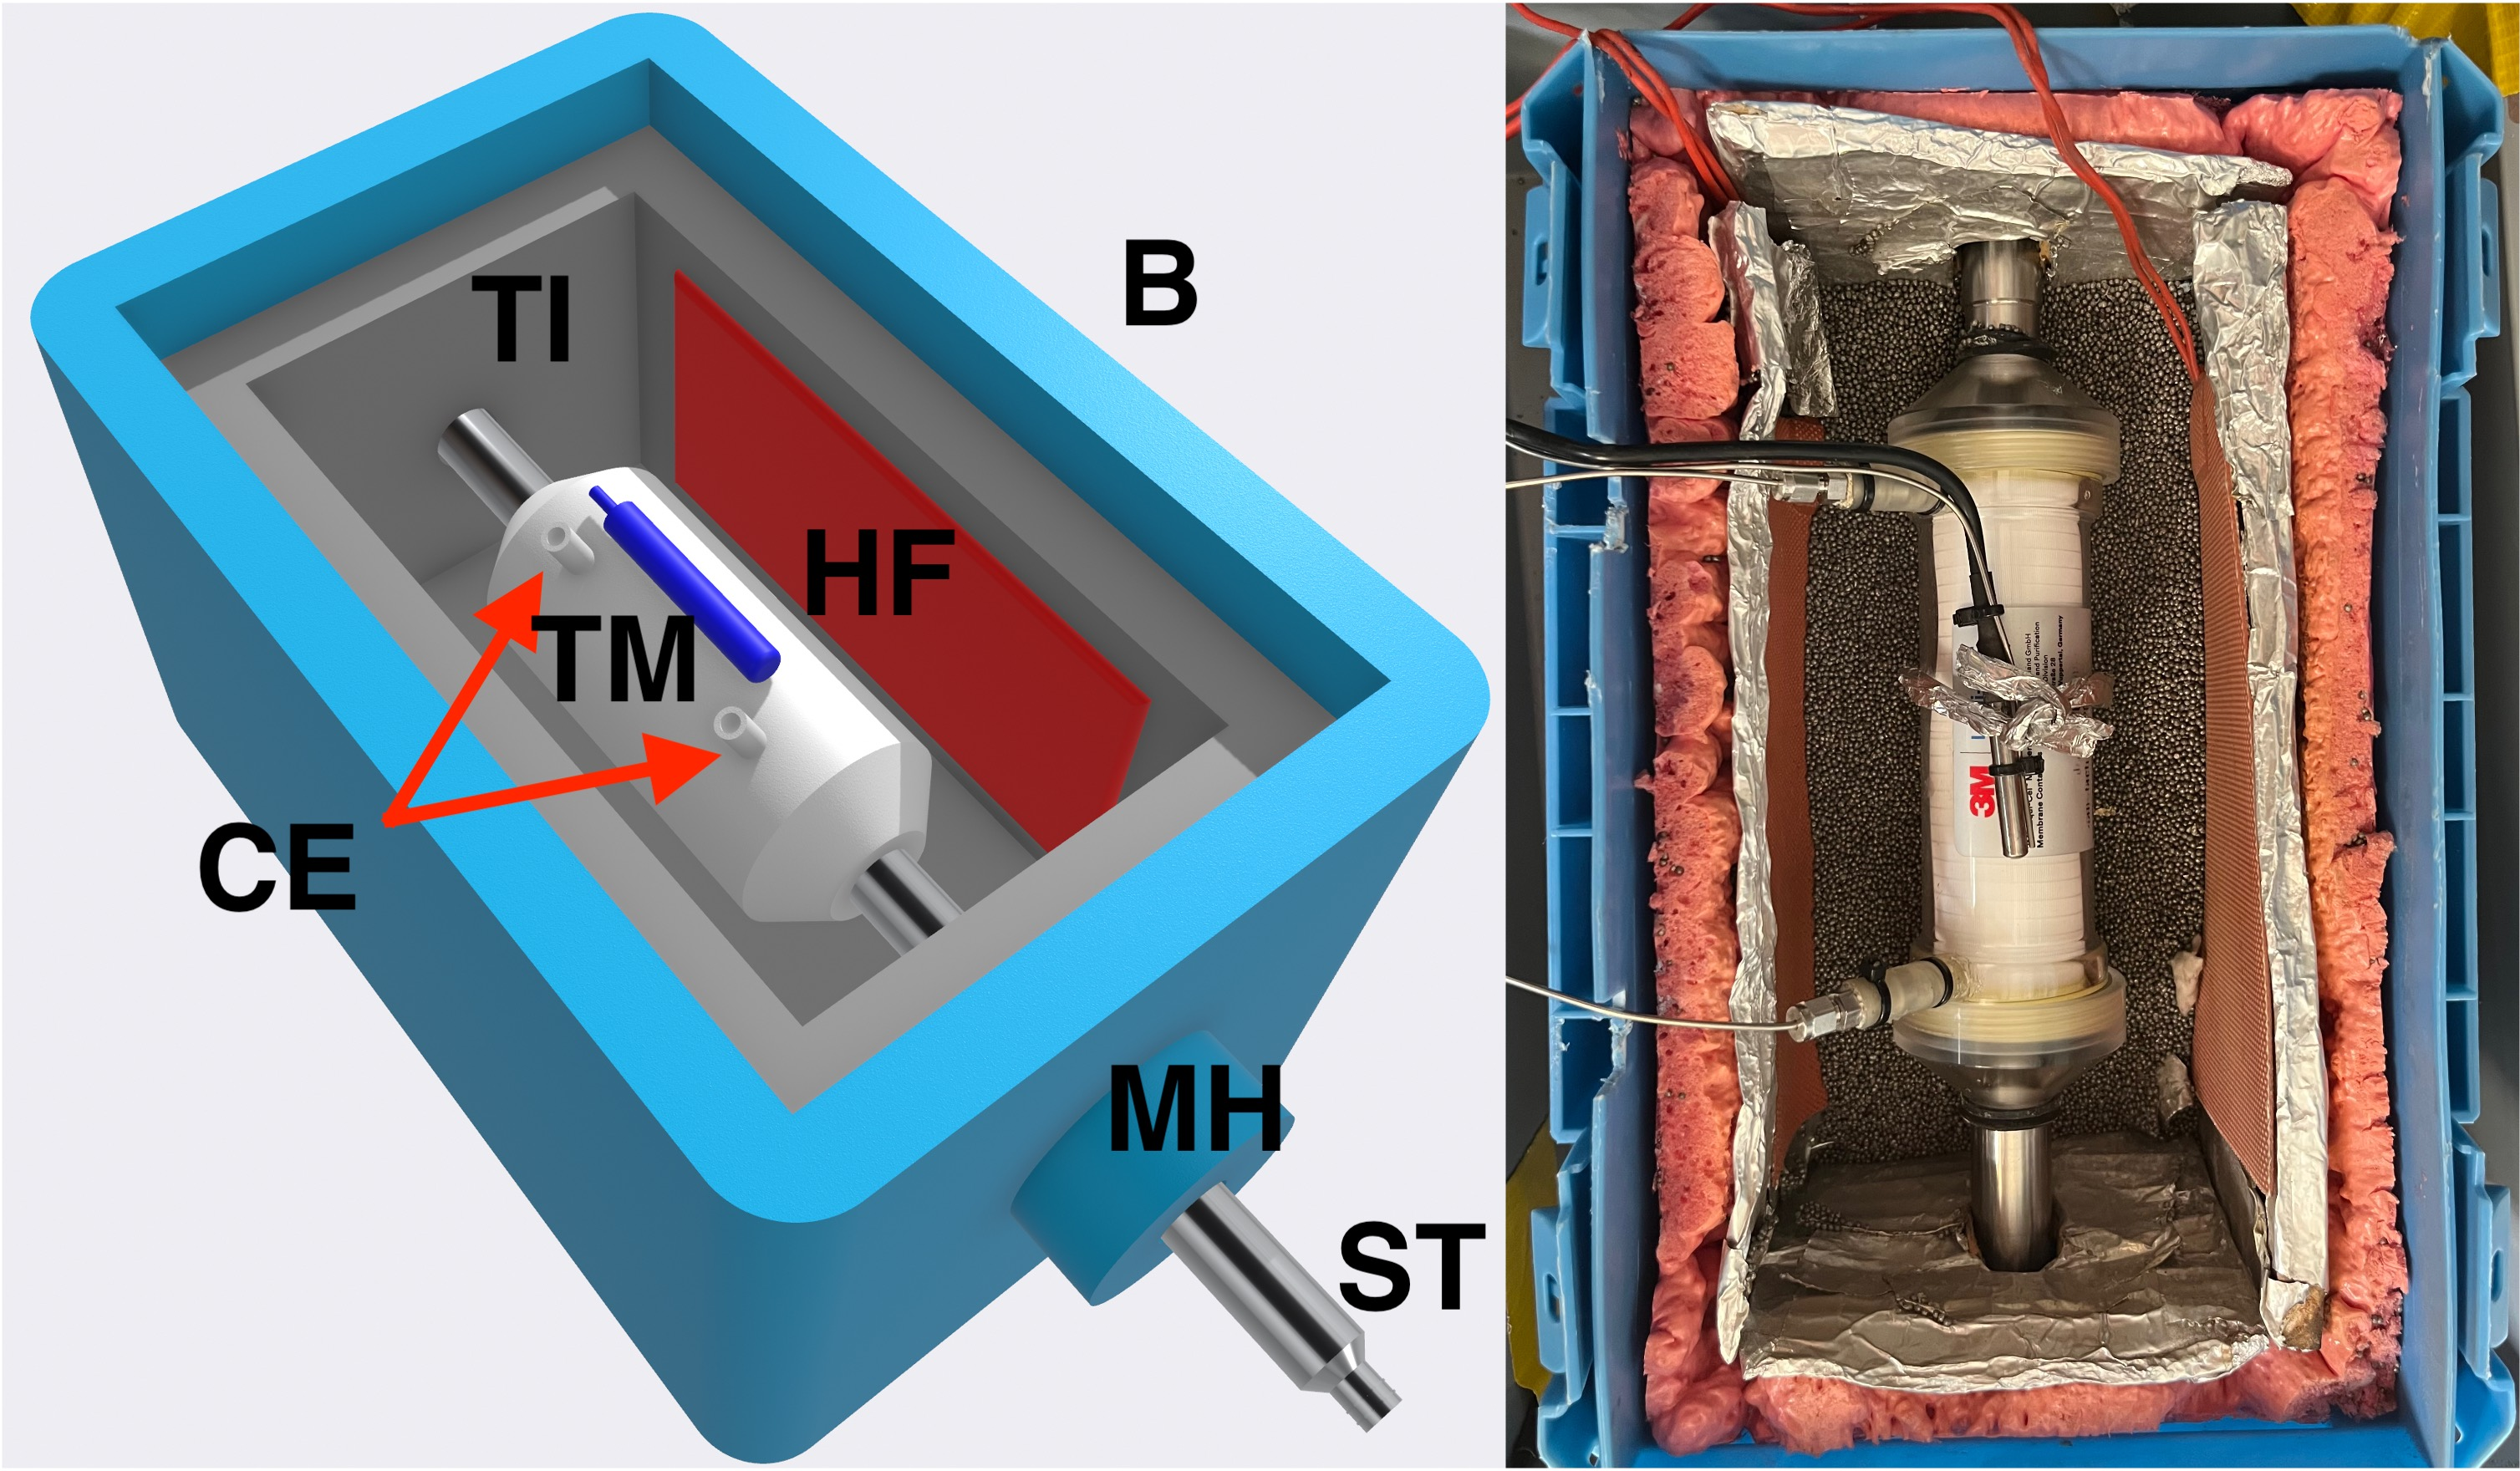
\includegraphics[width=1\textwidth]{chapters/02_chap1/figures/figure_1.jpeg}
\end{center}
\caption{
Heating box for moderate temperature ranges of up to \SI{65}{\celsius}. 
The box (B) is thermically isolated (TI) and the void space is filled with metal castings. 
This provides a constant high temperature to the membrane module (MM).
The heating foils (HF) heat the castings to a predefined temperature (i.e., above the temperature of the water/fluid being analyzed).
The temperature is monitored by two thermometers (TM, represented by the blue part in the schematic view).
The first belongs to the thermostat, while the second is monitored by the control unit to ensure that the temperature does not fall below the threshold. 
Two steel tubes (ST) are connected to the membrane module and circulate the thermal water.
Water is entering on one side, passes through the gas permeable membrane inside the module, and exits on the other side.
Mechanical stresses on the membrane module were reduced by mechanical holds (MH) which distributed forces to the box rather than to the membrane module. 
Two capillary entries (CE) allow to measure the partial pressure of individual gas species in the headspace of the MM, whose gas phase is in equilibrium with the dissolved gases in the liquid phase under analysis. 
}
\label{fig:1}
\end{figure}

One approach to quantify gas species in thermal waters without condensation of water vapor, and related clogging, is heating the membrane module to a temperature higher than the analysed water.
For this purpose, a heating box (see Fig.~\ref{fig:1} for a schematic view) was designed and built. 
The heating box was thermally isolated (see Fig.~\ref{fig:1}, TI), and three heating foils (see Fig.~\ref{fig:1}, HF) were placed inside to provide heat to maintain the heating box at the required temperature.
The empty space inside the heating box between the membrane module and the heating foils was filled with metal castings (e.g., 1.25--\SI{1.70}{\mm}, AR101652, IEPCO), which resulted in efficient heat conductance in the box (i.e., rapid and homogeneous distribution of the thermal energy). 
This guaranteed a homogeneous temperature at the surface of the membrane module.
The temperature inside the heating box was controlled and monitored by two thermometers (see Fig.~\ref{fig:1}, TM).
The first temperature sensor was part of a self-made thermostat, which supplied power to the heating foils to ensure that the temperature inside the heating box remained constant and at a sufficiently high value to avoid water vapor condensation.
The second temperature sensor was directly monitored by the control unit of the miniRUEDI to detect any failure of the heating box, such as a lower temperature (e.g., due to a shortcut in the heater foils), which would lead to water vapor condensation in the analytical system.
If the temperature in the heating box fell below a predetermined temperature threshold (which was set \SI{3}{\celsius} higher than the temperature of the monitored water), the control unit would disconnect the membrane module from the gas analyzer.
This was achieved by changing the gas inlet to a dead-end port.

We note that the commercially available membrane modules are built from polymers (polycarbonate), which limits their application to hydrothermal waters up to \SI{65}{\celsius} (a maximal heating temperature of \SI{70}{\celsius} was reached during a three-month test before failure of the membrane module).
Although most polymers do have a melting point higher than \SI{100}{\celsius}, the plastic tends to weaken when exposed to heat.
Any mechanical stress (e.g., torsional and weight forces of the connected water supply lines) promotes cracks and thus damages the structure of the membrane module.
Highly strained parts, such as screw threads of the water inlet and outlet of the membrane module, are particularly affected.
To avoid the early malfunctioning of the inlet and outlet, the hard plastic fittings supplying the membrane module with water were replaced with custom stainless steel fittings at a later stage during monitoring. 
These stainless steel tubes (see Fig.~\ref{fig:1}, ST) were held by cylindrical hard structures attached to the outside of the heating box (see Fig.~\ref{fig:2}, MH), which were designed to reduce mechanical stresses on the membrane module by holding the stainless steel tubes and distributing mechanical stresses on the hard box rather than on the membrane module.
To the authors' best knowledge, no suitable commercial alternative was found, as the more robust membrane modules were too expensive, rather large, and had the disadvantage of having a steel surface, making it impossible to observe the water level in the headspace in case of water vapor condensation. 

\subsection{Geothermal fluids over 65\textcelsius }\label{sec:high} 
Geothermal fluids in active hydrothermal fields can easily exceed \SI{65}{\celsius}, and the monitoring of gas species in these fluids cannot be accomplished by the first method covered in the previous section, calling for an entirely different approach to the problem posed by water vapor condensation within the membrane module.
At site 2, the high water temperature (close to boiling temperature) precludes the use of the membrane module for gas--liquid separation.
Thus, to monitor the gas composition at site 2, we decided to optimize our analytical techniques to gases continuously emitted from the outlet of a water/steam separator which is directly connected to the well head.
Gas species are quantified from the gaseous phase (i.e., gases emitted by the thermal water) and not directly in the liquid phase. 
We designed a system to draw the gases from the outlet of the separator towards the inlet of the portable mass spectrometer (see Fig.~\ref{fig:2}).

\begin{figure}[h!]
\begin{center}
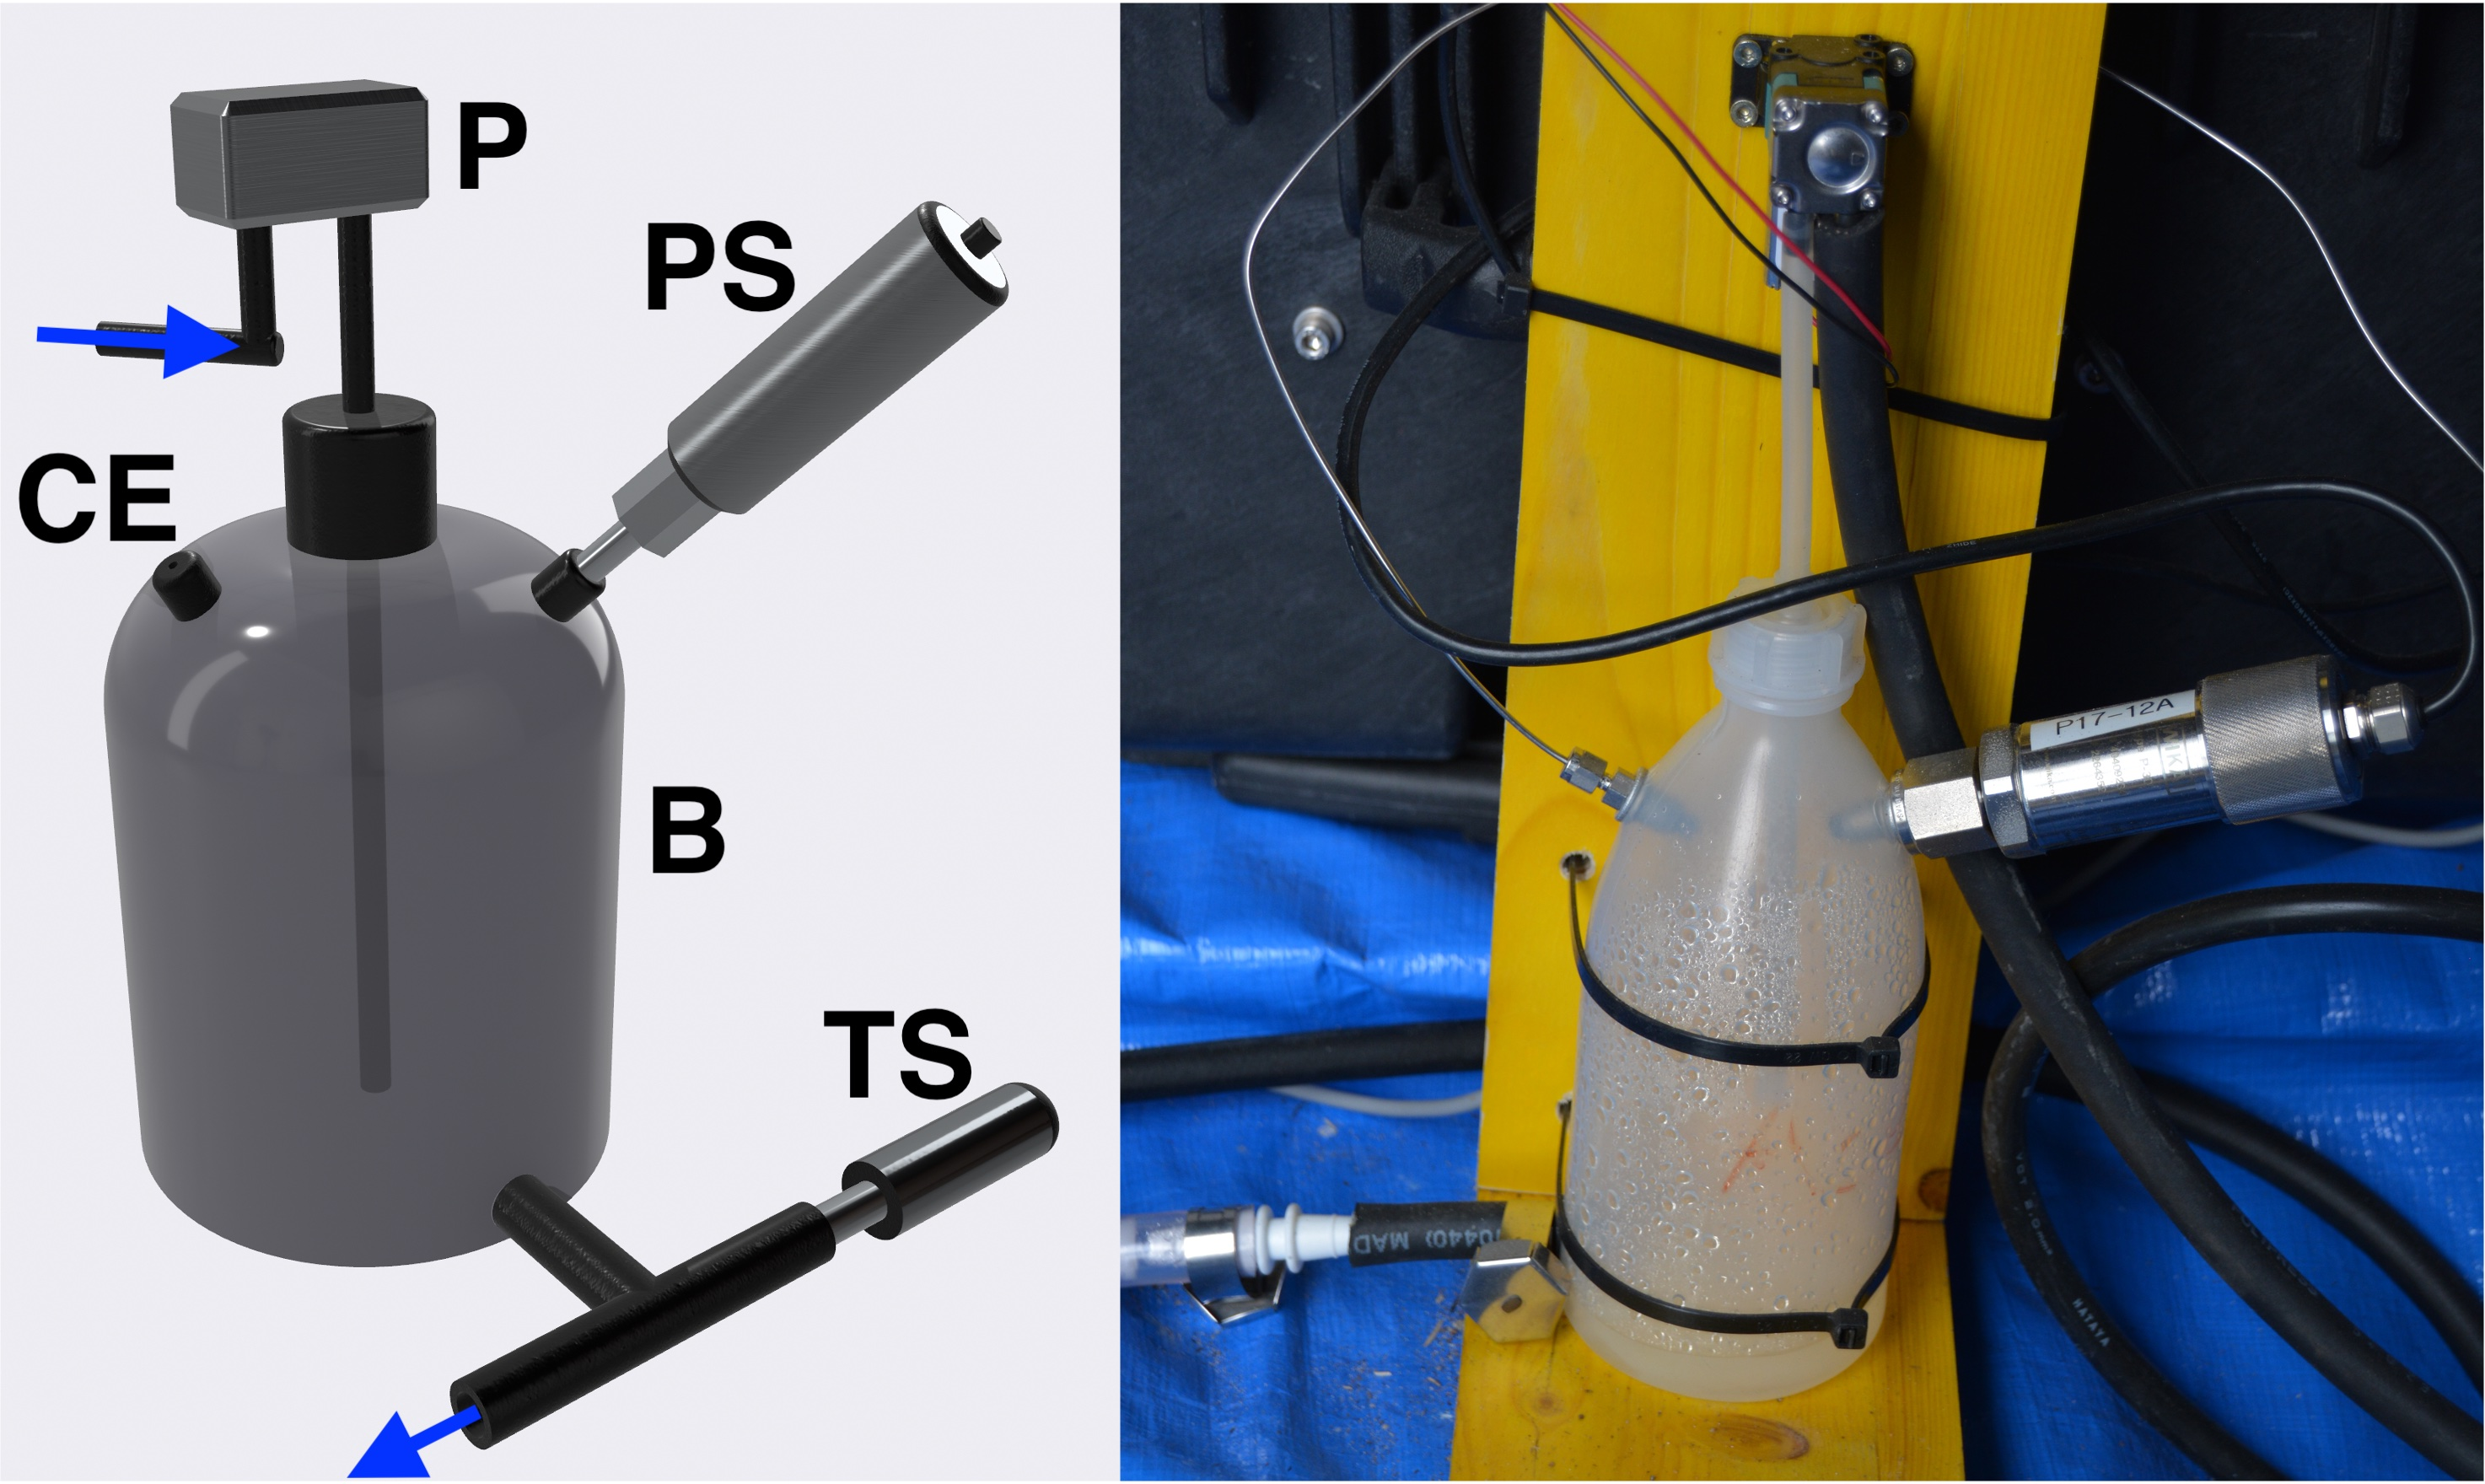
\includegraphics[width=0.9\textwidth]{chapters/02_chap1/figures/figure_2.jpeg}
\end{center}
\caption{Sampling bottle for fluid temperatures superior to \SI{65}{\celsius}.
A motorized pump (P) pumps the hot fluids (e.g., water vapor) into the bottle (B).
Two sensors measure the temperature (TS) and the pressure (PS) of the pumped gas.
A capillary entry (CE) allows to measure the gases using the miniRUEDI. 
As incoming gases and condensed water vapor are forced into the bottle near the bottom, condensation-related clogging of the analysis system is avoided because the gas analyzer inlet is located on the upper side of the bottle.
}
\label{fig:2}
\end{figure}

A \SI{10}{\m}-long ethylene propylene diene monomer rubber tube (gas-tight) withstanding temperatures of up to \SI{105}{\celsius} was inserted for approximately \SI{0.5}{\m} into the metal outlet of the separator.
The other end of the rubber tube (heat resisting synthetic rubber, POLYPRESS, \SI{9.5}{\mm} inner diameter) was connected to a pump (KNF, model FF 20 DC-M KT, see Fig.~\ref{fig:2}, P) equipped with PTFE membranes (fluoropolymer).
The pump circulated the liberated gases at a flow rate of $\SI{210}{\milli\litre\per\min}$ through an attached plastic bottle (volume $\SI{500}{\milli\litre}$, see Fig.~\ref{fig:2}, B).
The residence time of the gases in the rubber tube was sufficient to cool the gas phases close to ambient temperature.
Therefore, most of the water vapor condensed within the rubber tube.
The inlet of the plastic bottle was designed so that liquid water was prevented to reach the capillary inlet at the top of the bottle. 
A tube carried gases and liquid water from the top towards the bottom of the bottle, releasing fluids at the bottom of the bottle (see Fig.~\ref{fig:2}).
The chosen design and the used pumping rate allowed the complete mixing of the headspace in the bottle due to temperature gradient and turbulent fluid flow.
A total gas pressure sensor were connected in the upper part of the bottle (see Fig.~\ref{fig:2}, CE and PS, respectively).
An outlet for both gaseous and liquid phases was set at the bottom of the plastic bottle.
The temperature changes of the fluids were monitored by a temperature sensor (see Fig.~\ref{fig:2}, TS) at the outlet of the bottle.

\section{Results and discussion}
\subsection{Method for water temperatures below 65\textcelsius}
At site 1, the self-made heating box was tested on two different water temperatures.
In an early test phase, the method was tested on a hydrothermal well where thermal waters reach a temperature of \SI{62}{\celsius} at the well head.
Therefore, the heating box had to be set at a constant temperature of approximately \SI{70}{\celsius}. 
In this first test phase, measures to reduce the mechanical stress on the membrane module were not implemented, leading to a total failure of the membrane module when the inlet walls failed after three months. 
Nevertheless, this test phase showed the potential to monitor thermal waters up to \SI{65}{\celsius}, as the heating box provided sufficient energy to remove water vapor condensation from the headspace of the membrane module. 

For operational reasons and due to the annual shutdown of the deepest and hottest well at site 1, the setup, which has been additionally improved to reduce mechanical stresses on the membrane module, was transferred and installed to the shallowest well (P201, \SI{201}{\mbgl}), where the thermal waters reach a temperature of \SI{52}{\celsius}.
The temperature threshold for the heating box was set to \SI{55}{\celsius} and the thermostat to \SI{58}{\celsius}.
The temperature threshold was never reached, which ensured that the temperature inside the box was always higher than the water temperature during the experiment.
As of August 2022, the monitoring of gas species from the thermal waters abstracted from the well P201 has been ongoing for 12 months. 
During the 12 months of operation, the membrane module showed no signs of water condensation nor total failure. 
The developed heating box successfully heated the membrane module to avoid condensation.
In addition, the physical support provided by the mechanical holds (see Fig.~\ref{fig:2}, MH) significantly extended the lifespan of the membrane module (three months for the first test phase, over 12 months for the currently ongoing experiment).

Given that the monitoring of gas species was successful because of the proper functioning of the heating box, we could process some preliminary results to illustrate what could be achieved by monitoring gas species in thermal waters. 
Data were filtered to include only measurements at temperatures higher than \SI{48}{\celsius}.
Data points at lower temperatures were measured while the pump was inactive and are therefore not representative of the targeted water.
Figure~\ref{fig:3} shows the complete time series of gas concentrations (approximately one measurement every \SI{15}{\minute}, resulting in over \SI{2600}{} individual data points for each gas species, with concentrations expressed as gas partial pressures being at equilibrium with the dissolved gas phase in the thermal water) taken at the well P201 during October 2021.
\ce{N2}, Ar, \ce{O2}, Kr, He, \ce{CH4}, \ce{CO2}, and \ce{H2} partial pressures were simultaneously quantified from the thermal water using integrated procedures from the miniREDI system \citep{brennwald2016portable}.
The data were smoothed (Savitzky-Golay filtering, frame length 27 and order 3).
The major gas was \ce{N2}, which accounted for approximately \SI{96}{\percent} of the total gas pressure.
Ar, He, and \ce{CH4} were the following most abundant gases, with each accounting for approximately 1--\SI{2}{\percent} of the measured total pressure. 
\ce{O2}, Kr, \ce{H2}, and \ce{CO2} accounted for the rest of the measured gas fraction. 

\FloatBarrier % Ensure previous floats are placed before proceeding

\afterpage{% Delays the figure until the next page
\clearpage
\begin{figure}[p]
\begin{center}
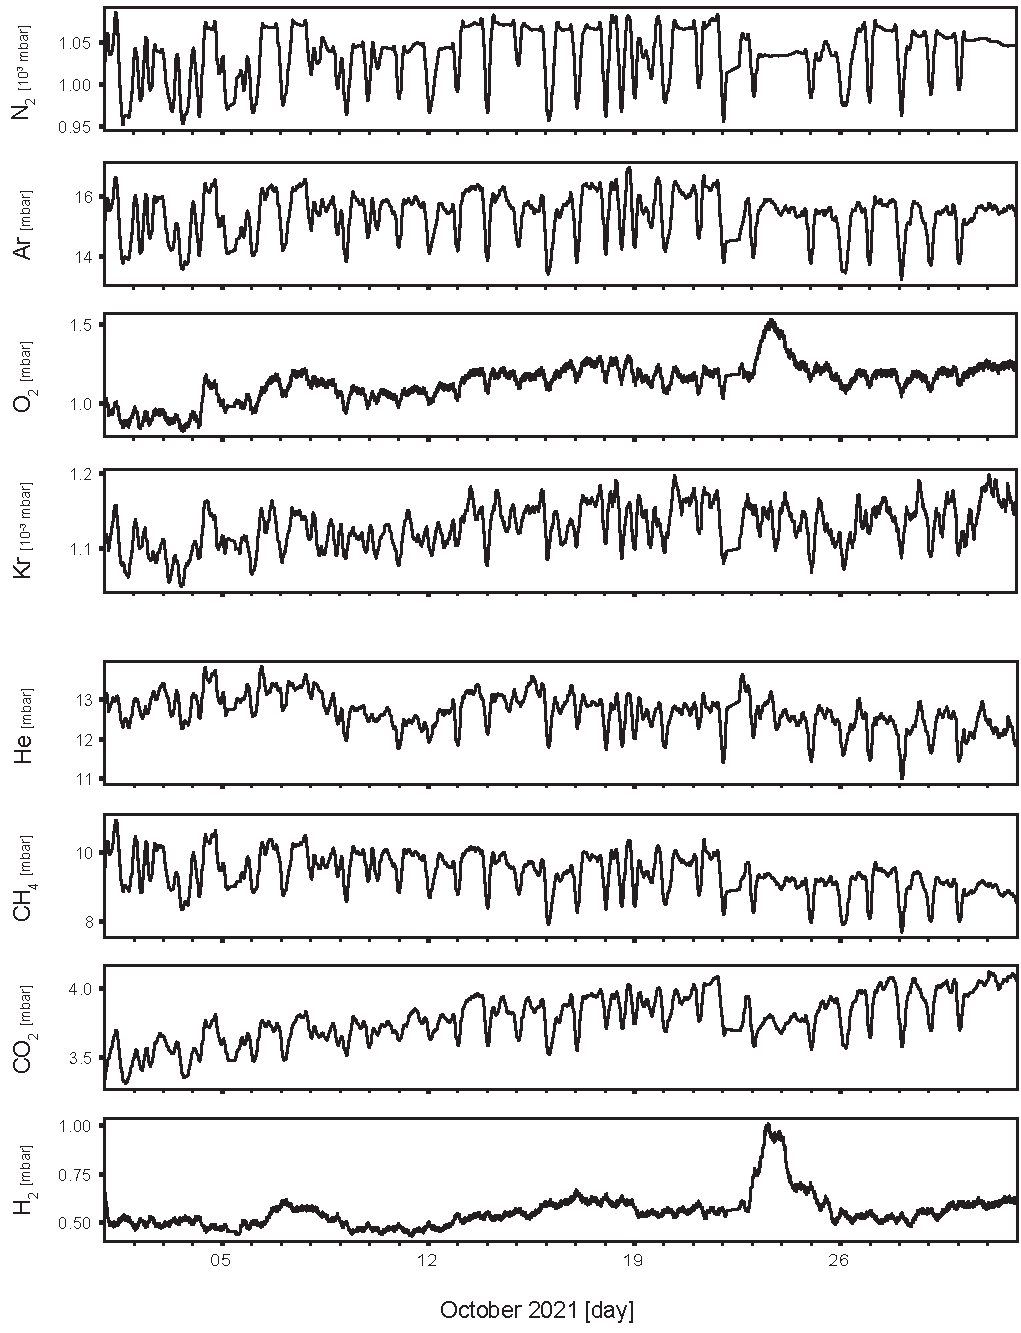
\includegraphics[width=0.9\textwidth]{chapters/02_chap1/figures/figure_3.pdf}
\end{center}
\caption{Time series of gas measurements ($>2600$ data points) conducted at Lavey-Les-Bains (Switzerland) in October 2021.
The determined partial pressures [mbar] of \ce{N2}, Ar, \ce{O2}, Kr (atmospheric gases), He, \ce{CH4}, \ce{CO2}, and \ce{H2} (geogenic gases) are plotted using Savitzky-Golay filtering (frame length 27 and order 3) to smooth the curves.
On October 22, the P201 pump was offline for a duration of \SI{8}{h} due to an operation failure. 
The different peaks in the shaded area, such as those in the concentrations of \ce{H2} and \ce{O2}, are possible effects of the pumping interruption.}
\label{fig:3}
\end{figure}
\clearpage
}

During October 2021, the gas composition evolved in time while short (hours to day) and long (week to month) trends were observed. 
All gas measurements showed distinct short-term oscillations with a frequency of about one day.
These short-term oscillations can most likely be related to the different pumping rates of well P201 to supply thermal water to the local spa (hot water requirements were greater during the day when the spa was open to the public than at night).
Superimposed on the short-term variations, gas concentrations appeared to vary gradually during October 2021 (e.g., slow decrease of \ce{CH4}, slow increase of \ce{CO2}).
Whether these long-term variations were also related to the pumping regime or whether they reflect the natural variability of the dissolved gases in the thermal water of Lavey-les-Bains is the subject of ongoing research \citep{giroud2022monitoring}.
Recording short- and long-term trends in the temporal evolution of gas species in thermal waters (see Fig.~\ref{fig:3}) would hardly have been possible without the use of the new method developed to extend the applicability of continuous monitoring of gas species to warm waters up to \SI{65}{\celsius}.

\subsection{Method for fluid temperatures over 65\textcelsius}
At site 2, the method was implemented to analyze the gas composition in fluids reaching the boiling temperature of water.
During the two months of operation, the separation of the high water vapor content from the rest of the gases never compromised the gas detector responsible for monitoring the gas species from the hot fluids, as the liquid water was flushed out of the bottle and never reached the critical level to clog the analysis system (i.e., the height of the capillary connecting the bottle to the gas detector).
As no membrane module is required in this approach, the only limiting factor for the quantification of gas species in thermal fluids was given by the thermal resistance of the rubber tube.
The rubber tube must be long enough to cool fluids close to room temperature, allowing water to condense inside the rubber tube, and must be able to withstand the high temperature of the fluid.
Once again, the data provided when using the method at site 2 during the monitoring of gas species from thermal fluids is valuable in illustrating the range of possibilities that can be achieved with this new method. 

Figure \ref{fig:4} shows the results of the gas measurements conducted in April 2018 at the hydrothermal well at site 2.
The time series of the partial pressures of Ar, He, \ce{N2}, \ce{CO2}, \ce{CH4}, and \ce{H2} are reported together with concurrent seismic events occurring in the surrounding region.
The gas measurements were smoothed by filtering (see above).
\ce{CO2} and \ce{N2} were the most abundant gas species with partial pressure approximately \SI{850}{\milli\bar} and \SI{150}{\milli\bar}, respectively.
\ce{CH4} and \ce{H2} showed alternating phases of low and high concentrations, correlating with the temporal evolution of \ce{CO2} and \ce{N2}.
Phases of enhanced concentrations of \ce{H2} matched rather well with the timing of increasing \ce{CO2} concentrations, suggesting the deep origin of \ce{H2}, whereas high \ce{CH4} concentrations tended to correlate with the timing of increasing atmospheric gas concentrations.
Ar concentrations correlate well with \ce{N2} concentration measurements, whereas He concentrations seemed to correlate neither with major changes in \ce{CO2} nor with major changes in \ce{N2} concentrations, although being slightly enriched with respect to atmospheric air.

\begin{figure}[H]
\begin{center}
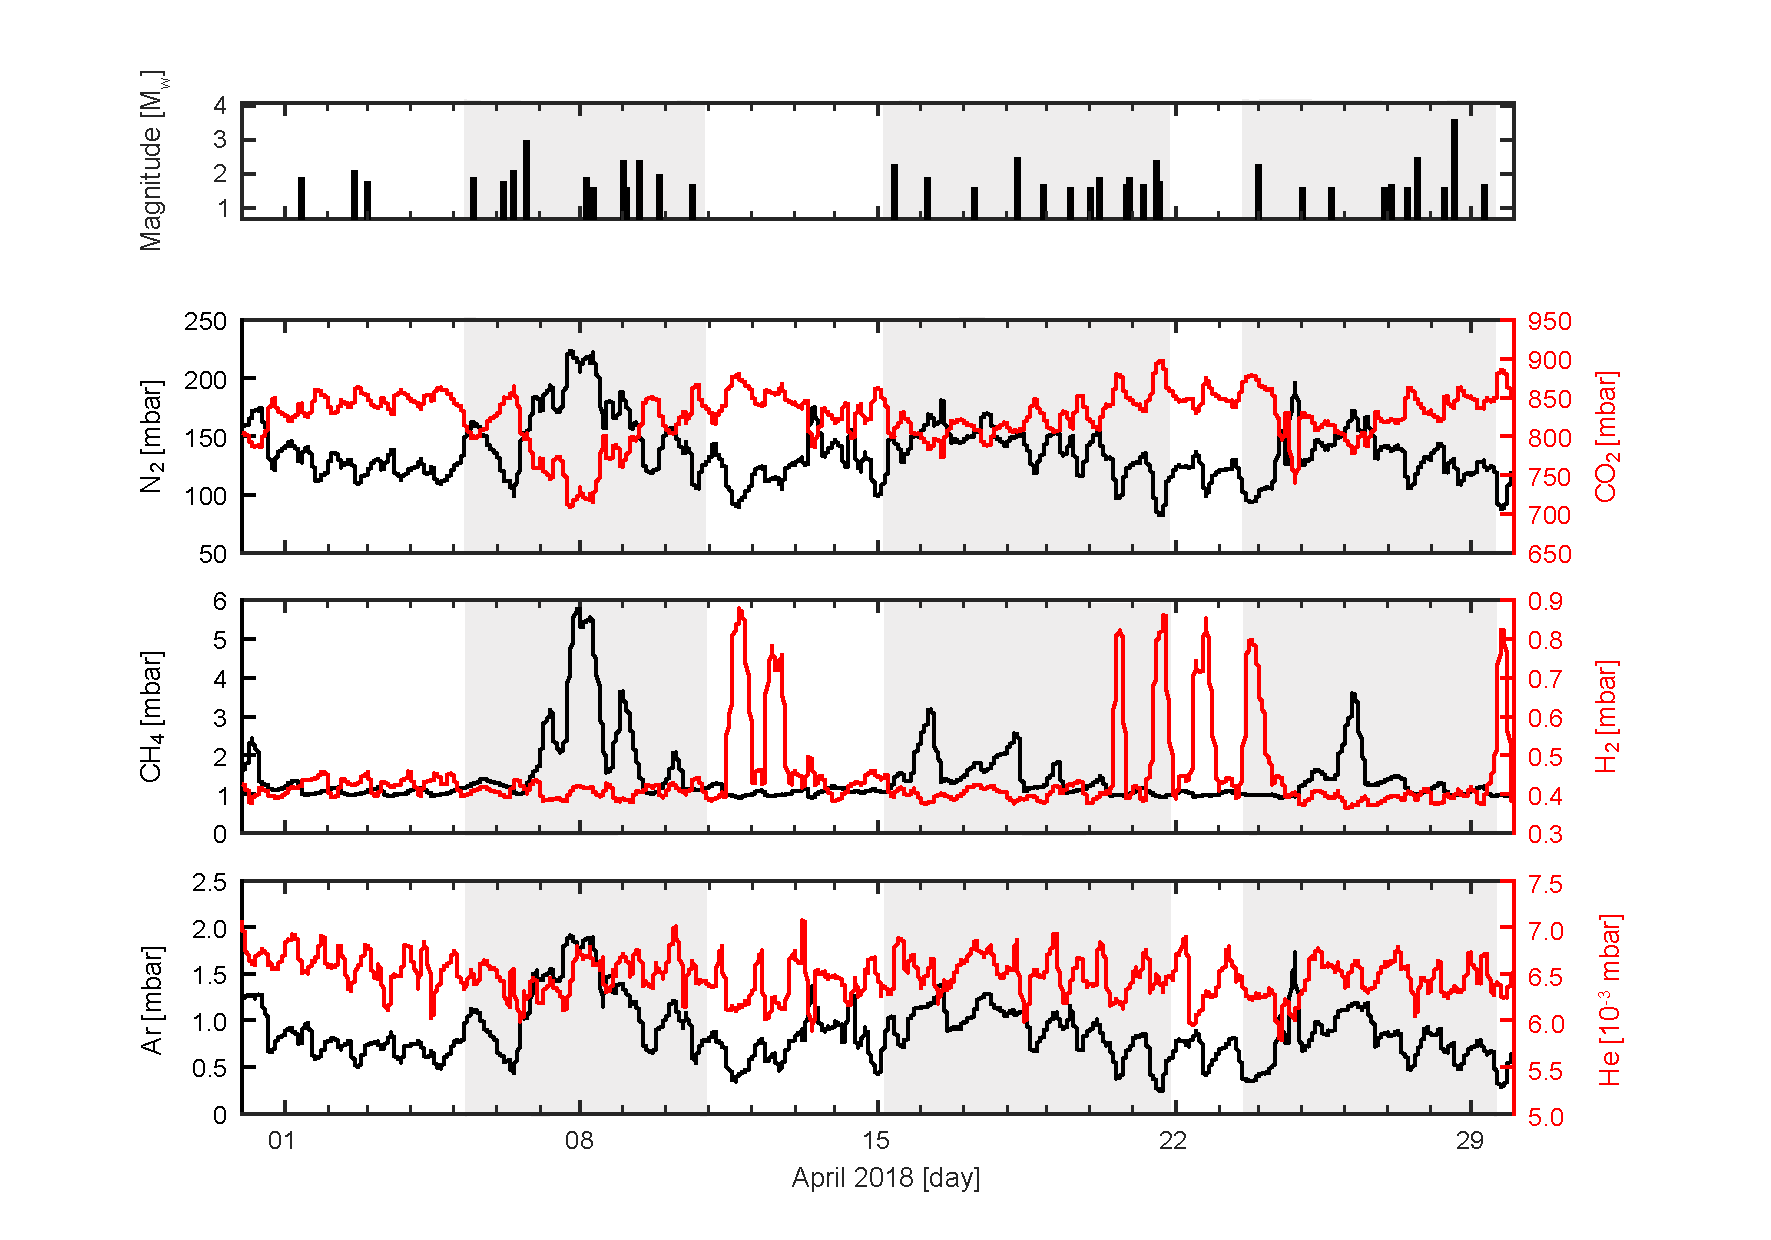
\includegraphics[width=1\textwidth]{chapters/02_chap1/figures/figure_4.pdf}
\end{center}
\caption{Time series of gas measurements ($> 2000$ data points) conducted in April 2018 at the hydrothermal well in Beppu (Japan).
The upper panel indicates phases of low (white) and of higher (grey) seismic activity. 
The lower panels show gas species whose long-term temporal variation are either anti- (e.g., \ce{N2}-\ce{CO2} or \ce{CH4}-\ce{H2}).
Mid-term changes as seen for \ce{N2} and \ce{CH4} can be seen in the Ar time series. 
He does not seem to be affected by low or higher seismic activities. 
As for Fig.~\ref{fig:3}, a Savitzky-Golay filtering (frame length 27 and order 3) was used to smooth the curves.
}
\label{fig:4}
\end{figure}


These observations suggest that a mechanism modulates the mixing of a deep-sourced gas component (enriched in \ce{CO2} and \ce{H2}) and a shallower gas component (carrying atmospheric gases, such as \ce{N2} and Ar, but possibly also \ce{CH4} from a surface-near source).
A solid statistical analysis of the relation between geochemical changes and seismicity cannot be achieved in the context of this work as the amount of data is very limited. 
Nevertheless, the data suggest that the peak concentration of \ce{CH4} synchronously occurs with more active seismic phases (upper panel of Fig.~\ref{fig:4}).
Conversely, phases of high \ce{H2} concentrations appear during time periods of lower seismic activity.
Other hydrothermal sites in seismically active regions are currently being studied to explore the possible relation between seismicity and fluid dynamics \citep{giroud2022monitoring}.

\section{Conclusions}
Increasingly, efforts to monitor environmental conditions call for robust and portable technologies.
In the case of thermal fields where high temperature water is close to the earth's surface, gas analyzers, especially those relying on capillary inlets, can be impacted by the high water vapor content and the associated risk of water vapor condensation.
The two methods we presented in this study allow us to extend the on-site analytical methods for gas quantification, such as the miniRUEDI, for geothermal applications.

Both methods open new experimental possibilities to study the temporal and spatial variability of gases in thermal waters and hot terrestrial fluids (e.g., fumaroles), that are notoriously difficult to assess by conventional sampling methods, which rely on the analysis of a few individual samples.
Our developed methods are a step forward for the systematic analysis of the possible relation of terrestrial fluid dynamics and seismicty in volcanic and tectonic active regions \citep{giroud2022monitoring}.
Similarly, the developed methods open a new analytical window to track fluids in the context of deep-rock experiments (i.e., by labeling water with a noble gas as an artificial tracer, \cite{zappone2021fault, roques2020helium}).


\cleardoublepage